\subsection{Cross-Side Request Forgery (Buchberger)}
\label{sec:content_security_xsrf}
\paragraph{Problem}
Folgende Situation:\\
Ein Super-Admin (nennen wir ihn Bob) ist in SIS eingeloggt, solange er das Browser-Fenster nicht schließt bleibt die PHP-Session aufrecht. \\
Nun öffnet er in einem anderen Browser-Tab versehentlich die Website von Marvin (Marvin kennt die SIS-Seite, und er kennt den Source-Code). Marvins Seite fragt mit AJAX die SIS-Seite an. Er füllt mit JavaScript das Formular zum Löschen der Stundenpläne aus und sendet es zurück. Da diese Anfrage mit Bobs Webbrowser ausgeführt wird, und dieser eine offene PHP-Session mit SIS hat, glaubt das SIS-System, dass die Anfrage von Bob kommt. Resultat sind unerwünschte Änderungen in der Datenbank.\\
Nun, ganz so funktioniert es nicht, da Domain-übergreifende (\enquote{Cross-Origin-Access}) AJAX-Requests vom Browser üblicherweise unterbunden werden. Nicht unterbunden wird das Laden von iFrames auf Marvins Seite, der Webbrowser lässt auch hier den Zugriff auf das iFrame durch JavaScript nicht zu (siehe \autoref{fig:content_security_xsrf0}).\\
Jedoch kann Marvin nun im Hintergrund seiner Seite ein Formular aufbauen, das die selben Felder enthält, wie das SIS-Formular, das er manipulieren will. Als target-Frame für das Fomular gibt er das iFrame an. Die Daten werden an das iFrame gesendet und von SIS verarbeitet.\\
Diese Technik wird \enquote{Cross-Side Request Forgery} - kurz XSRF - genannt.

\begin{figure}[H]
\centering
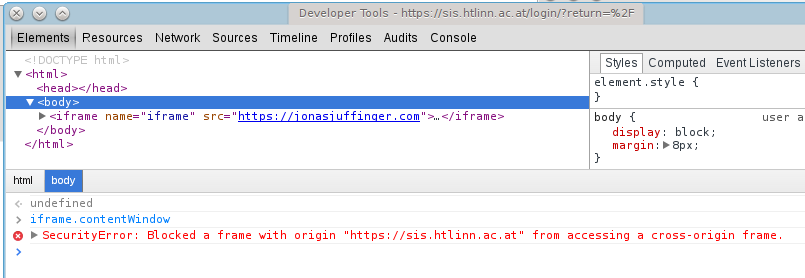
\includegraphics[keepaspectratio=true, width=14cm]{images/screenshots/xsrf0.png}
\caption{Browser blockiert Cross-Origin-Access auf iFrame}
\label{fig:content_security_xsrf0}
\end{figure}
\paragraph{Methoden um Vorzubeugen}
Es gibt einige Möglichkeiten, um diesem Problem vorzubeugen:
\begin{itemize}
	\item Die einfache Möglichkeit ist das Überprüfen des Referer-Feldes im HTTP-Kopf. Bei solchen XSRF-Angriffen wird üblicherweise das Referer-Feld auf die Seite des Angreifers umgeändert. Jedoch sollte man sich nicht auf dieses Feld verlassen, da viele Privatsphäre-Browser-Plugins  das Mitsenden dieses Feldes verhindern. Auch können Proxy-Server und ähnliches dieses Feld verändern.
	\item Über das HTTP-Feld \texttt{X-Frame-Options: SAMEORIGIN} wird der Webbrowser angewiesen nur das Einbinden über Seiten mit dem gleichen Ursprung zu erlauben. Dieses Feld ist jedoch noch nicht bei allen Browsern implementiert, so sollte man sich nicht darauf verlassen.
	\item Die gängigste Variante, um dieses Sicherheitsproblem zu entfernen ist, eine zufällig generierte Zeichenkette an jedes Formular anzuhängen. Dieser Hash ist mit der PHP-Session verknüpft und authorisiert in gewisser Weise den Inhalt. In Fachkreisen wird oft von \enquote{Page-Token} oder von \enquote{Nonce} gesprochen. Der Angreifer hat - unter Annahme, der Webbrowser funktioniert ordnungsgemäß - keine Möglichkeit dieses Token auszulesen. Diese Möglichkeit verwenden wir auch bei SIS (siehe \gref{sec:content_draft_vsession}).
\end{itemize}